\documentclass[a4paper, 12pt]{article}

\usepackage{geometry}
\geometry{a4paper,
total={170mm,257mm},left=2cm,right=2cm,
top=1cm,bottom=2cm}
\usepackage{wrapfig}
\usepackage{graphicx}
\usepackage{mathtext}
\usepackage{amsmath}
\usepackage{siunitx} % Required for alignment
\usepackage{multirow}
\usepackage{gensymb}
\usepackage{rotating}
\sisetup{
  round-mode          = places, % Rounds numbers
  round-precision     = 2, % to 2 places
}

\usepackage[T1,T2A]{fontenc}

\usepackage[russian]{babel}

\graphicspath{{pictures/}}


\title{\begin{center}Лабораторная работа №2.2.6\end{center}
Определение энергии активации по температурной зависимости вязкости жидкости.}
\author{Каграманян Артемий, группа Б01-208}
\date{\today}

\begin{document}

\maketitle

\section{Аннотация}
\textbf{Цель работы:} Измерение установившейся скорости падения шариков в вязкой жидкости в зависимости от ее температуры. Рассчет вязкости жидкости по формуле Стокса и нахождение энергии активации.\\
\\
\textbf{Оборудование:} стеклянный цилиндр с исследуемой жидкостью, термостат, секундомер, горизонтальный компоратор, шарики.\\
\\
\textbf{Теоритическая справка:} В жидкости каждая молекула находится в потенциальной яме электрического напряжения, которое создается из-за окружающих молекул. Средняя кинетическая энергия молекул меньше, чем глубина этой ямы, так что молекулы колеблются относительно более или менее устойчивых положений равновесия. Но так как разность между ними мала, молекулы могут совершать движение между потенциальными ямами. Чтобы перевести молекулы из одного состояние в другое, им нужно придать тепловую энергию \(W\), которая называется энергия активации. Вязкость жидкости в небольших интервалах можно выразить как:
\[\eta \sim Ae^{\frac{W}{kT}},\]
где $k$ - константа Больцмана, $A$ - безразмерная величина. Изобразив график \(ln \eta\) от \(\frac{1}{T}\), получится прямая, описывающая прямую \(ln\eta = lnA + \frac{W}{kT}\), через угловой коэффициент которой можем найти \(W\). Рассмотрим, какая сила сопротивления действует на шарик. Она зависит от нескольких параметров, но при выводе величины этой силы с помощью метода размерности, можем понять:
\[F = A\eta r v\]
Нахождение коэффициента \(A\) очень сложно, поэтому воспользуемся формулой Стокса, где \(A = 6\pi\). Теперь, через формулу Стокса и второй закон Ньютона, можем найти \(\eta\):
\[\rho V \frac{dv}{dt} = (\rho - \rho_{ж})g V - 6 \pi \eta r v\]
\[v(t) = v_{уст} + (v(0) - v_{уст})e^{-\frac{t}{\tau}}\]
\[\eta = \frac{2}{9}gr^2\frac{\rho - \rho_ж}{v_{уст}}, \ v_{уст} = \frac{Vg(\rho - \rho_ж)}{6\pi r \eta}, \tau = \frac{6\pi r \eta}{\rho V}\]
Таким образом, нам нужно определить установившиеся скорости шариков при разных температурах жидкости, в результате чего мы сможем найти \(\eta\), а потом и \(W\).
\section{Описание экспериментальной установки} 
\begin{figure}[h]
    \centering
    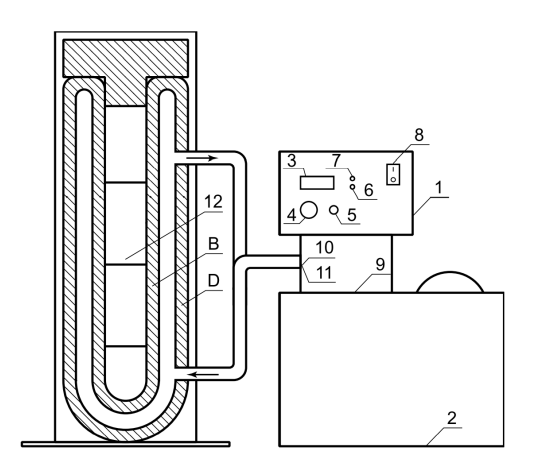
\includegraphics[width=0.5\linewidth]{226pic.png}
\end{figure}
Температура исследуемой жидкости задается термостатом. На трубке, в которой она находится, есть верхняя метка (она расположена так, чтобы шарики после ее прохождения падали с постоянной скоростью) и нижняя метка. Мы секундомером замеряем время падения шарика от одной метки до другой. Также нам нужно замерить диаметры шариков и усреднить их значение для каждого (чтобы увеличить точность эксперимента, так как шарик не принимает идеальную сферическую форму). Температуры для экспериментов будем брать из интервала между комнатной температурой и 50-60\(\degree C\).

\section{Данные, их обработка и получение результата}
Возьмем 20 шариков и будем их кидать в глицерин (по 4 шарика в глицерин определенной температуры), замеряя время, за которое шарик проходит от метки до метки. Так как время релаксации много меньше времени прохождения шарика расстояния между метками, без разницы, от какой метки начинать отсчет (их там 3). Получаются следущие значения:
\begin{figure}[h]
    \centering
    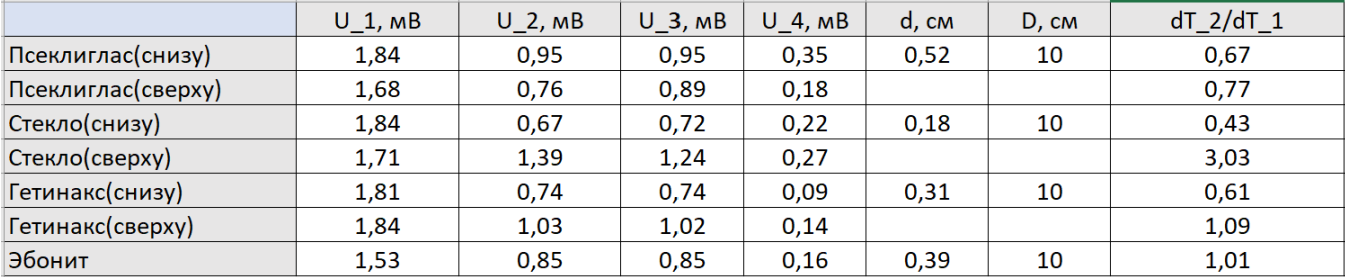
\includegraphics[width=0.8\linewidth]{data.png}
\end{figure}
\newpage
Для каждого значения можем посчитать коэффициаент динамической вязкости по формуле из теор. справки (в таблице также указана и погрешность):

\begin{figure}[h]
    \centering
    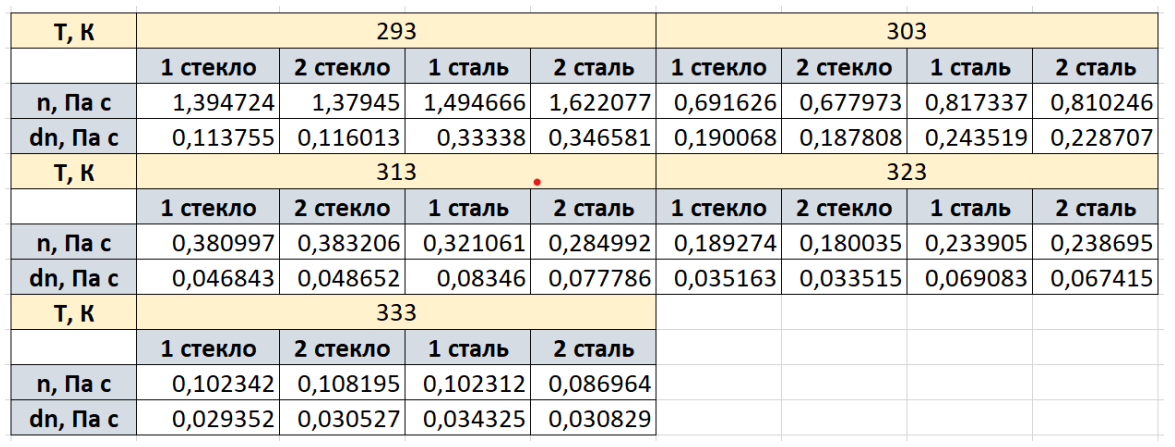
\includegraphics[width=0.8\linewidth]{prepared.png}
\end{figure}
При вычислении этих значений было учтено, что плотность глицерина меняется с температурой.
\\
\\
По этим данным нам нужно построить график зависимости \(ln \eta\) от \(\frac{1}{T}\):
\begin{figure}[h]
    \centering
    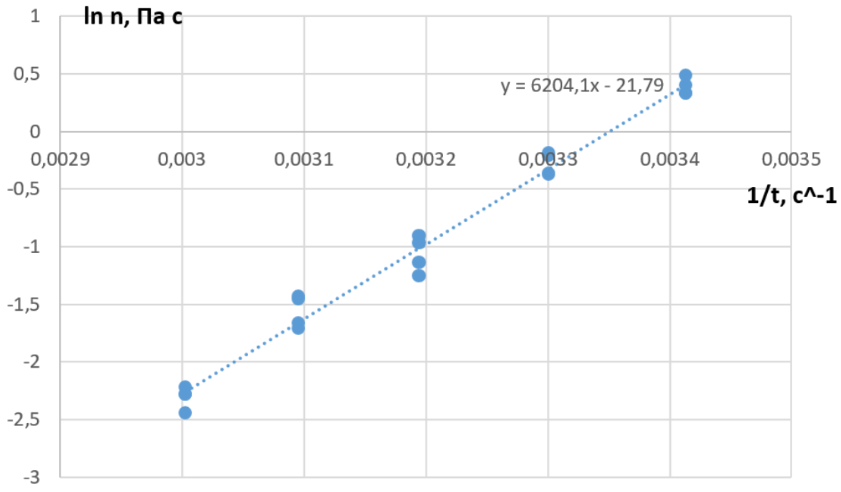
\includegraphics[width=0.8\linewidth]{plot.png}
\end{figure}

Угловой коэффициент аппроксимирующей прямой равен \(W/k\), откуда мы получаем значение энергии активации. Итого, получилось:
\[W = 0.53 \pm 0.3\ Эв\]
\section{Заключение}
Мы получили коэффицикенты взякости для глицерина при различных температурах, а затем и значение энергии активации. Оно получилось не такое, как табличное (спасибо кривым рукам экспериментаторов), но порядок получился такой же.
\end{document}
